\chapter{Evaluation}
\label{chapter:evaluation}

This chapter discusses the methodology, configuration, and results of an experimental evaluation comparing the performance of the PBTC, SCATS, and Vehicle Actuated traffic control strategies implemented within PBTSim. Performance evaluation and analysis is required to determine the effectiveness and appropriateness of the PBTC system. Evaluation was carried out within the developed PBTSim application to measure and analyse the impact of control strategy heuristics with regards to incurred delays and costs imposed on vehicles within a simulation.

\section{Methodology}

Performance evaluation of traffic control methodology is made difficult by the proprietary and commercial nature of traffic control algorithms and the software systems that implement them. Section \ref{sec:scats_strategy} describes a number of design alternatives that were considered when implementing a representative SCATS system for evaluation. The chosen solution for the evaluation component of this project was designed to reconstruct a simulation of real-world SCATS behaviour using log files generated by SCATS containing phase times and traffic conditions of the SCATS system operating on intersections in Wellington over a 13-hour period. Previous research has similarly used SCATS log files for this purpose \cite{wolshon1999scats}.

Traffic demand on road networks is typically time varying, and the flow of traffic in urban centres typically peaks in the early morning and early evening periods, corresponding with commuters travelling to and from workplaces within the city, to urban or suburban residences. The 13-hour period of operation was determined with consideration to the typical profile of traffic in the central Wellington City area during a day, characterised by two peaks of high volume in the morning and evening for around 1--2 hours each. By evaluating traffic performance over a 13-hour period from 6:00 a.m. to 7:00 p.m., these peaks can be included in the evaluation, creating a range of traffic conditions for performance analysis. The log data used during evaluation was provided by the Wellington City Council (WCC), who operate SCATS for all of the intersections in the central Wellington City area. 

\section{Experimental Configuration}

The experimental configuration consisted of three simulated intersection configurations, based on real-world intersections within central Wellington City; namely the intersections of Vivian Street and Victoria Street, Victoria Street and Karo Drive, and Courtney Place and Tory Street. Appendix \ref{appendix:scats_intersections} includes a map showing the location of each intersection, and screenshots of the intersection configurations within SCATS and PBTSim. 

Traffic volume was simulated by parsing vehicle detections from SCATS log file for each of the three evaluation intersections. SCATS log files provided by the WCC contained 13 hours of data logged on Thursday 20th June, 2013. A static traffic composition configuration of 80\%/20\%, light vehicles/heavy vehicles was used for all of the simulation runs during evaluation.

Each simulation run was repeated ten times for each of the PBTC, SCATS, and Vehicle Actuated control strategies on each of the three evaluation intersections, for a total of 90 unique simulations. Post-processing tools were used to report the mean and standard deviation of results for each set of repeated runs. The set of results generated by each simulation run include the following evaluation metrics:

\begin{itemize}
\item Mean number of vehicle arrivals over each 30 second window of simulation
\item Mean delay time, cost of delay, and incurred costs of stopping for each vehicle during simulation
\item Delay time, cost of delay, and incurred costs of stopping of all vehicles over each 30 second window of simulation
\item Total delay time, cost of delay, and incurred costs of stopping for all vehicles during simulation
\end{itemize}

The Vehicle Actuated traffic control strategy was set to a fixed phase duration of 30 seconds, with minimum and maximum duration limits of 15 and 60 seconds, respectively. The gap timer duration was set to 3 seconds. Simulated detectors for the Vehicle Actuated strategy were placed 5 metres from the stop line. The geometric layout of each PBTSim intersection configuration was constructed to reflect the real-world geometry of each intersection, with lanes not used in the evaluation omitted. 

\section{Traffic Flow}
\label{sec:trafficflow}

To investigate the flow of traffic through the simulation networks over the course of the simulation period, the number of vehicle arrivals was logged every 30 seconds of simulation time. The flow of traffic over a 13 hour period during a typical day can be expected to vary, and the performance of different traffic management strategies may be affected by periodic flow rates. Traffic flow within the experimentation was generated from detector data contained within the SCATS log files of each intersection. Figure \ref{eval:vehiclearrivalstime} shows a plot of the trend in vehicle arrivals over the simulation period for each of the evaluation intersections. Each of the three intersections show evidence of ``peak'' traffic periods, typically during the first 3 hours and last 3 hours of the evaluation window.

The Vivian-Victoria intersection has significantly higher traffic flow than the other two intersections evaluated. As the inbound link of the southern motorway, Vivian Street is an arterial link of Wellington's road network and a typical route for many Hutt Valley and Porirua commuters working in the central business district (CBD). This is evidenced in \ref{vehiclearrivalstime:sub1}, flow recorded on the Vivian Street approach is considerably higher than Victoria Street for the majority of the evaluation window. The flow recorded at the Courtenay-Tory intersection is relatively low. As neither Courtenay Place or Tory Street are motorway approaches, the comparably lower rate of traffic flow is expected. 

The Karo-Victoria intersection shows clear evidence of morning and evening traffic peaks, with flow increasing up to the end of the evaluation period, which corresponds approximately 7 p.m. in real-time. As Karo Drive is the entry to the northern motorway, and one of the few routes by which Hutt Valley commuters can easily leave the CBD, the end-of-day flow increase is expected. The flow rate at the Victoria Street approach to the intersection remains consistently low over the entire evaluation period. In comparison to the Victoria Street flow at the upstream Vivian-Victoria intersection, this flow is unexpectedly low which suggests the SCATS log file may be incomplete (for example, due to a failed detector) and is not reflecting the real traffic flow at that intersection. 

\begin{figure}
\centering
\begin{subfigure}{.5\textwidth}
  \centering
  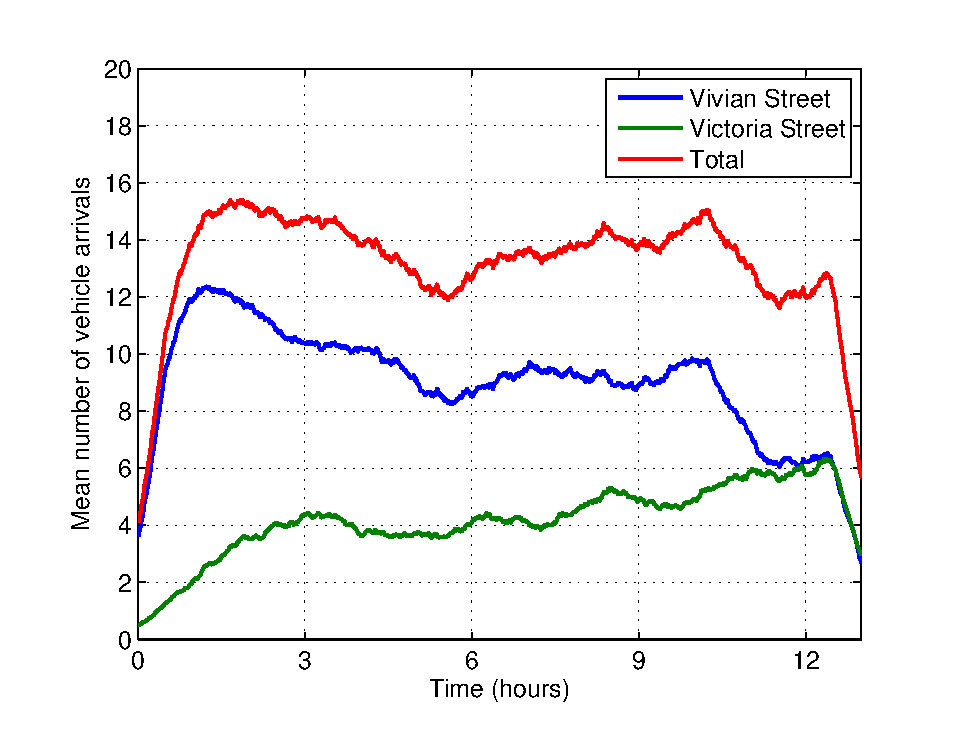
\includegraphics[scale=0.50]{vivian_victoria_num_arrivals_time.eps}
  \caption{Vivian-Victoria}
  \label{vehiclearrivalstime:sub1}
\end{subfigure}%
\begin{subfigure}{.5\textwidth}
  \centering
  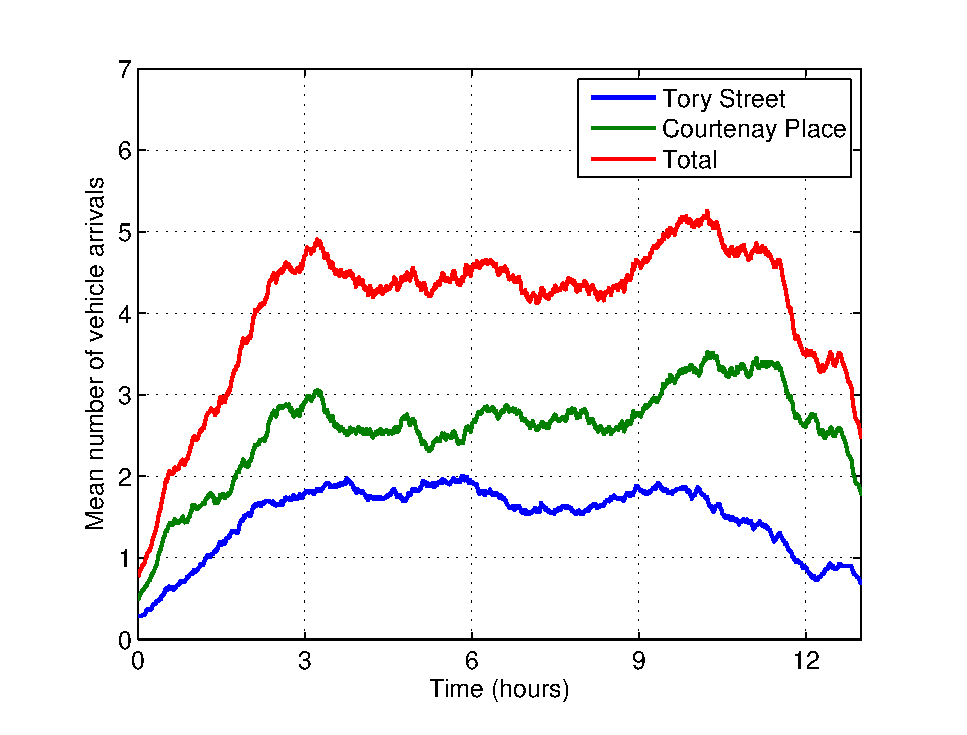
\includegraphics[scale=0.50]{courtenay_tory_num_arrivals_time.eps}
  \caption{Courtenay-Tory}
  \label{vehiclearrivalstime:sub2}
\end{subfigure}

\vspace{1cm}

\begin{subfigure}{.5\textwidth}
  \centering
  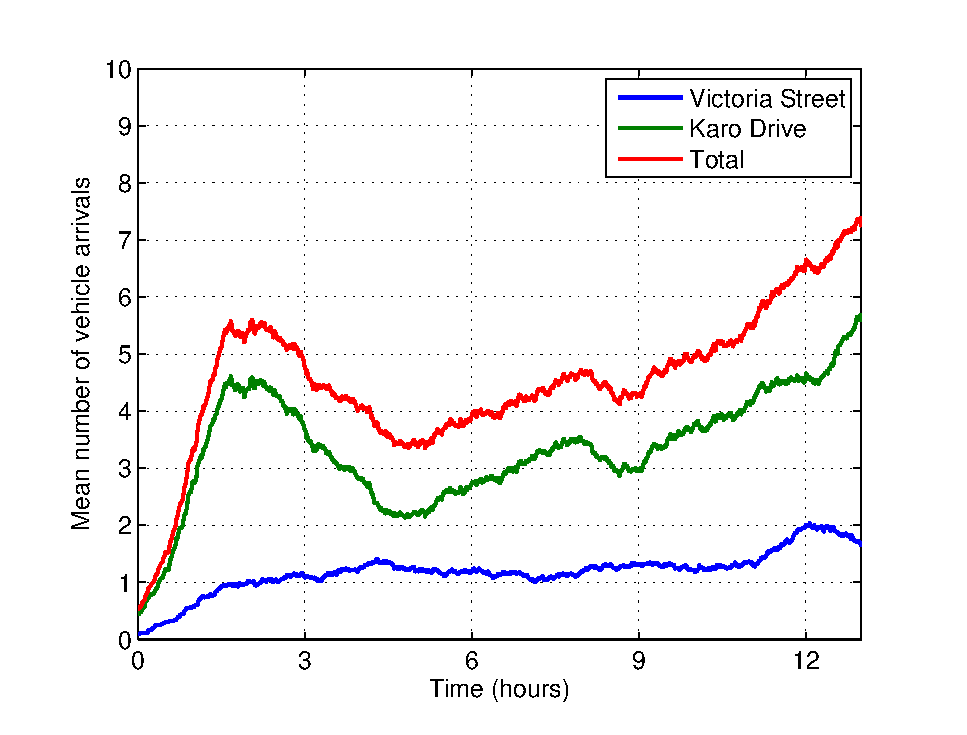
\includegraphics[scale=0.50]{karo_victoria_num_arrivals_time.eps}
  \caption{Karo-Victoria}
  \label{vehiclearrivalstime:sub3}
\end{subfigure}%
\caption[Results of measuring the mean number of vehicle arrivals for each intersection evaluated.]{ A plot of the trend in the mean number of vehicle arrivals per 30 seconds over the duration of the evaluation window of 13 hours for each of the evaluation intersections. The mean number of vehicle arrivals for each 30 second block is determined through use of a convolution filter to display a moving average per hour of simulation time. The filtered data effectively displays an overview of the trend of traffic flow at each hour of the evaluation window. The flow rate at all three intersections shows evidence of expected morning and evening peaks caused by worker commutes. }
\label{eval:vehiclearrivalstime}
\end{figure}

\section {Delay Time and Cost}
\label{sec:incurred_delay_cost}

Delay time and delay cost are related metrics, though the relationship is not directly proportional as the cost of delay for an individual vehicle is determined by a function of urgency as well as time. As the SCATS and Vehicle Actuated control strategies do not consider delay cost when making phase control decisions, the total time vehicles are delayed is a valuable metric for these two systems, and individual delay time is the most noticeable cost to road users at a controlled intersection.

Figure \ref{eval:approaches_delay_time} shows a plot of the mean time spent delayed by individual vehicles within the experimental simulation, distributed by vehicle urgency for each of the three control strategies evaluated. The PBTC control system is able to achieve lower mean delay times across each of the three intersections, most appreciably on the intersection of Karo Drive and Victoria Street. The Vehicle Actuated control strategy typically results in the longest mean delay times, although performance is improved over the SCATS control strategy on the Karo-Victoria intersection. A possible reason for this performance is that the fixed phase duration of the Vehicle Actuated strategy is appropriate for the traffic flow at this intersection. The SCATS controller consistently results in longer mean delay times across all vehicle urgencies for the Courtenay-Tory and Karo-Victoria intersections when compared to PBTC, and results comparable to PBTC for the intersection of Vivian Street and Victoria Street. 

The difference in mean delay time between the PBTC system and SCATS or Vehicle Actuated systems appears to be more pronounced on the Karo-Victoria and Courtenay-Tory intersections. One possible reason for this is the lower volume of traffic on each of these intersections, suggesting that the performance benefits of the PBTC system are higher in lower traffic volumes, as the PBTC controller can favour shorter phase durations to result in lower delay times. It is also possible that the reason for the degraded SCATS performance on the simulation of Karo-Victoria is due to an incomplete or non-representative log file, as described in Section \ref{sec:trafficflow}. 

The PBTC control system also shows evidence of urgency preference within the mean delay times recorded per urgency. There is a decreasing trend in mean delay times recorded by the PBTC control system for increasing urgencies, which reflects that the PBTC control system considers cost of delay as a function of time and urgency when making control decisions. The SCATS and Vehicle Actuated control strategies do not show any comprehensive evidence of this trend, as expected.
% note that there are significantly less priority 5 vehicles

\begin{figure}
\centering
\begin{subfigure}{.5\textwidth}
  \centering
  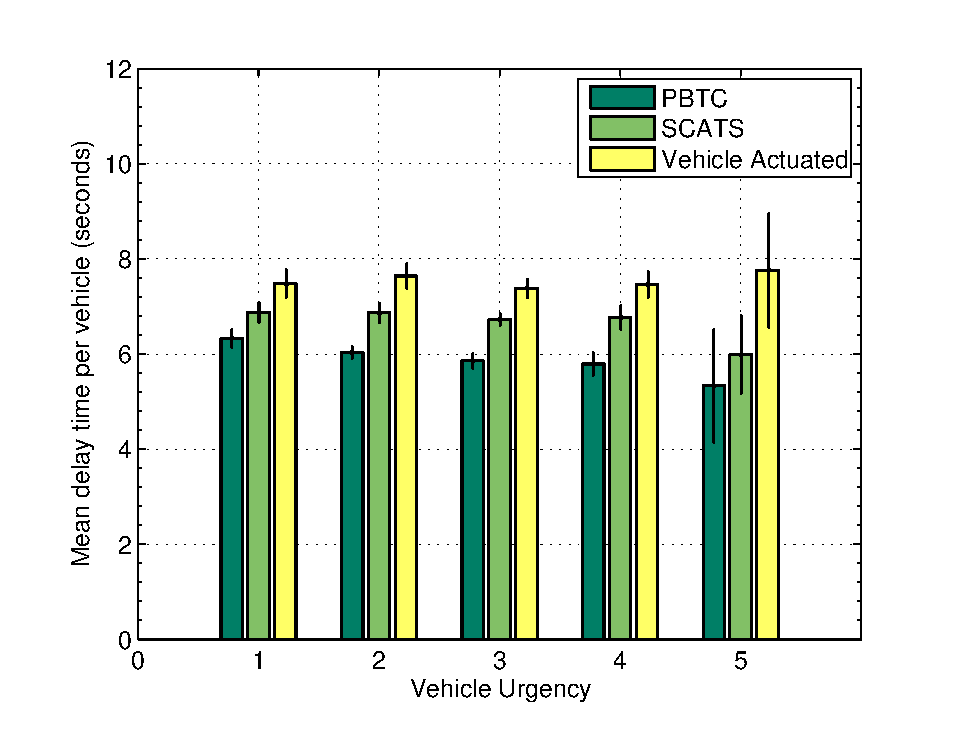
\includegraphics[scale=0.50]{vivian_victoria_approaches_delay_time.eps}
  \caption{Vivian-Victoria}
  \label{approaches_delay_time:sub1}
\end{subfigure}%
\begin{subfigure}{.5\textwidth}
  \centering
  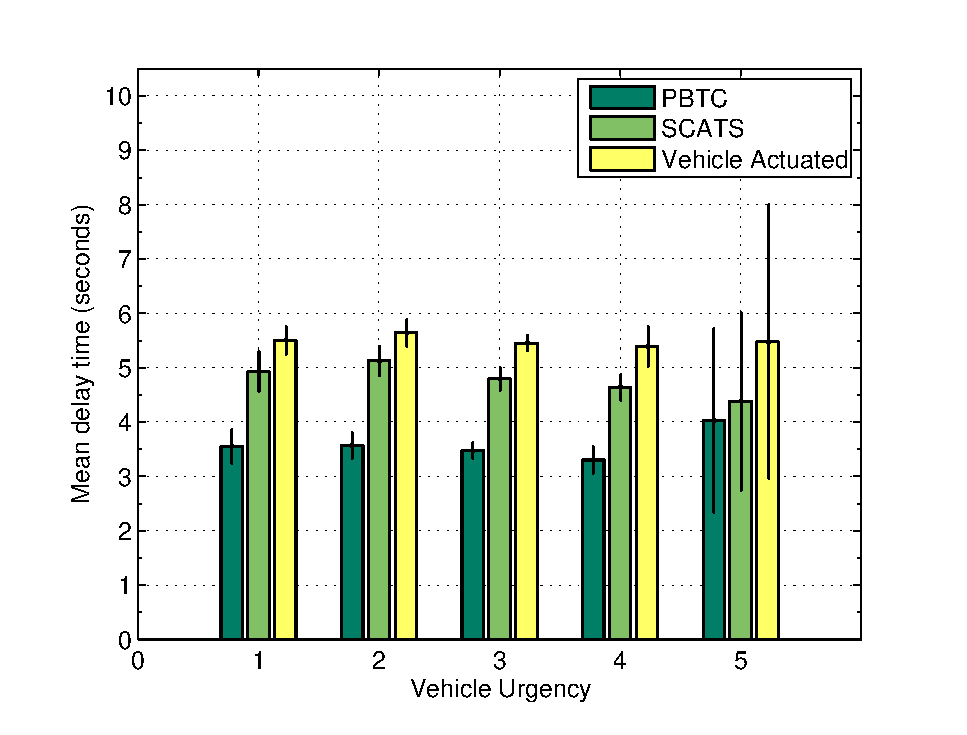
\includegraphics[scale=0.50]{courtenay_tory_approaches_delay_time.eps}
  \caption{Courtenay-Tory}
  \label{approaches_delay_time:sub2}
\end{subfigure}

\vspace{1cm}

\begin{subfigure}{.5\textwidth}
  \centering
  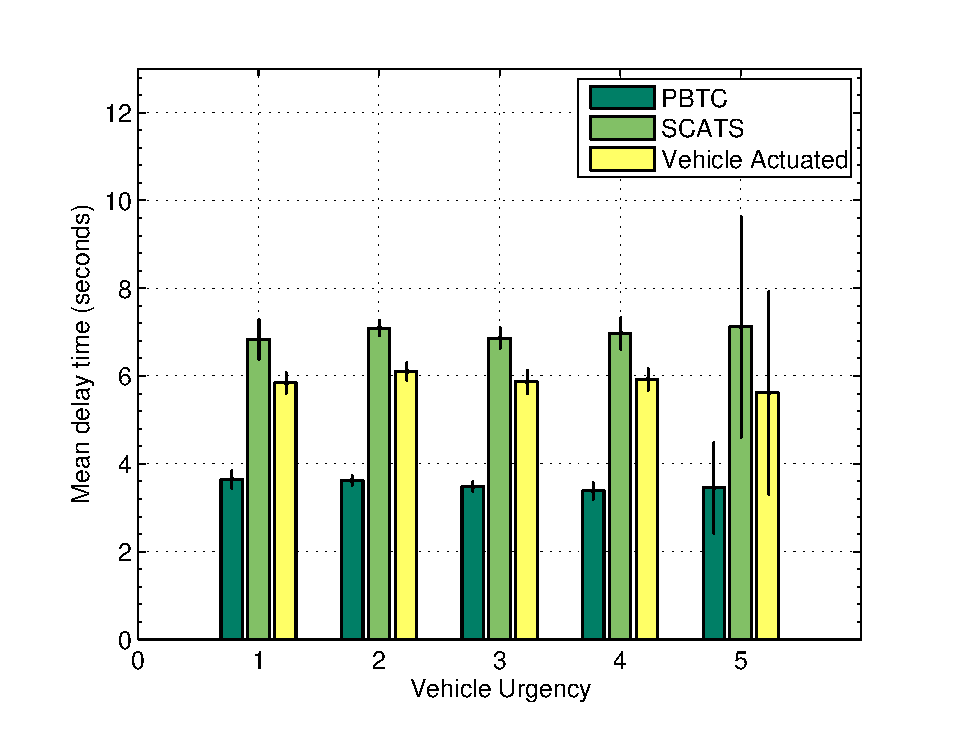
\includegraphics[scale=0.50]{karo_victoria_approaches_delay_time.eps}
  \caption{Karo-Victoria}
  \label{approaches_delay_time:sub3}
\end{subfigure}%
\caption[Results of measuring the mean delay time incurred by individual vehicles for each evaluation control strategy and intersection.]{ A bar chart of the mean delay time, measured in seconds, for an individual vehicle in the experimental simulation for each of the three evaluation intersections. Error bars shown are representative of a single standard deviation of the mean result. The PBTC control system outperforms SCATS and Vehicle Actuated controls over all of the dimensions.  }
\label{eval:approaches_delay_time}
\end{figure}

The PBTC system similarly outperforms the SCATS and Vehicle Actuated control strategies when considering the mean incurred cost of delay for individual vehicles within the experimental simulation. Figure \ref{eval:approaches_delay_cost} shows a bar chart of the delay cost, for each of the three control strategies and grouped by vehicle urgency. 

All three control strategies display a clear trend of increasing costs as vehicle urgency increases, expected as per the design of the delay cost measure, described in Section \ref{sec:design_delay_cost}. The PBTC control system consistently results in a lower mean delay cost for all vehicles in each simulation run. As with delay time, the Vehicle Actuated control strategy performs the worst with respect to delay cost over all three simulated intersections. From this result, we conclude that the fixed phase design of the Vehicle Actuated control strategy results in longer stopped durations and as a result a higher delay cost. The SCATS and Vehicle Actuated control strategies both perform significantly worse with respect to the cost of high urgency vehicles. Because the PBTC control system identifies and prioritises traffic based on urgency, the mean delay cost for higher urgency vehicles is relatively decreased.

 The standard deviation displayed on each of the charts is also more significant for urgency 5 vehicles. There are two possible reasons for this increased error; firstly, there are typically less than 5\% urgency 5 vehicles in each simulation as per the urgency distribution displayed in Table \ref{urgencydistribution}. Futhermore, as the relationship between time and delay cost for urgency 5 is greater, smaller differences in the delay time develop into larger delay costs and more significant error over a small sample.
 
\begin{figure}
\centering
\begin{subfigure}{.5\textwidth}
  \centering
  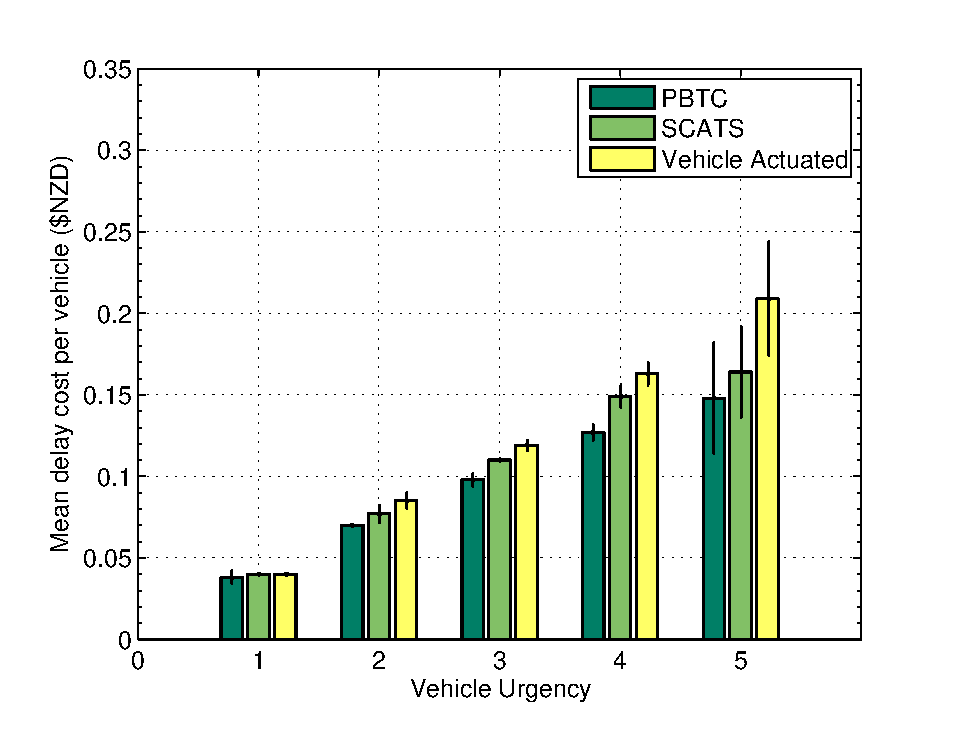
\includegraphics[scale=0.5]{vivian_victoria_approaches_delay_cost.eps}
  \caption{Vivian-Victoria}
  \label{approaches_delay_cost:sub1}
\end{subfigure}%
\begin{subfigure}{.5\textwidth}
  \centering
  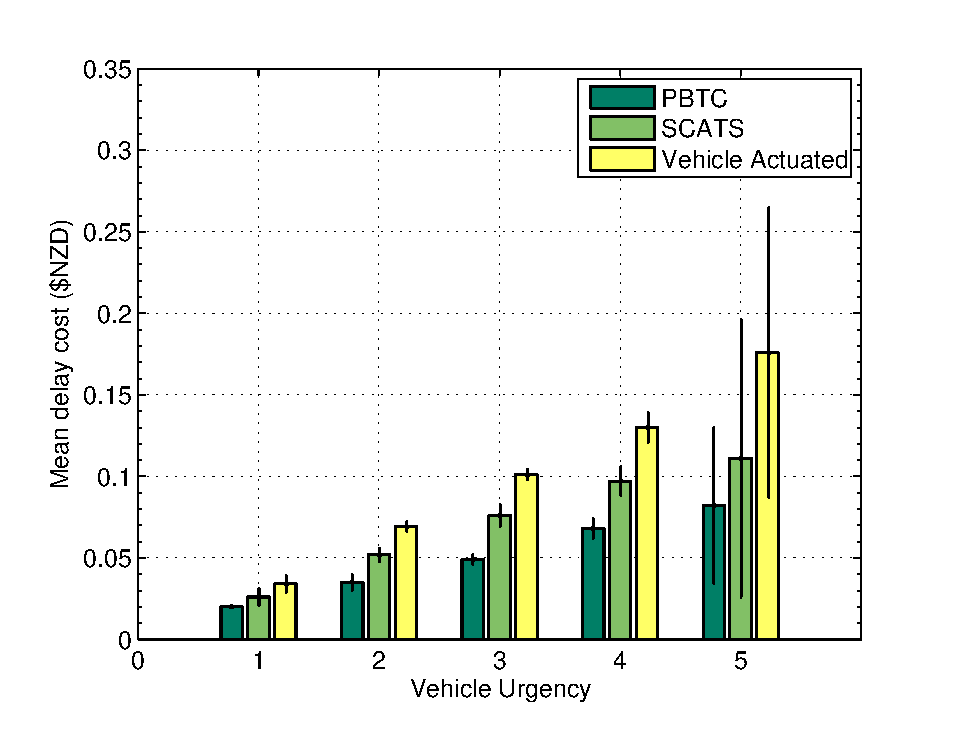
\includegraphics[scale=0.5]{courtenay_tory_approaches_delay_cost.eps}
  \caption{Courtenay-Tory}
  \label{approaches_delay_cost:sub2}
\end{subfigure}

\vspace{1cm}

\begin{subfigure}{.5\textwidth}
  \centering
  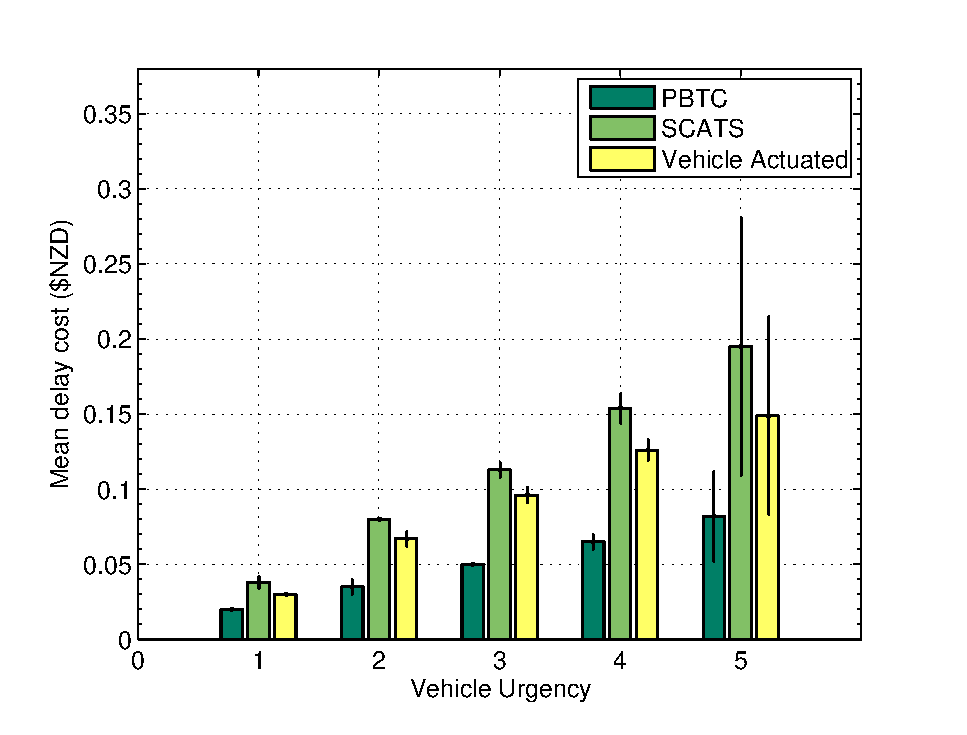
\includegraphics[scale=0.5]{karo_victoria_approaches_delay_cost.eps}
  \caption{Karo-Victoria}
  \label{approaches_delay_cost:sub3}
\end{subfigure}%
\caption[Results of measuring the mean delay cost incurred by individual vehicles for each evaluation control strategy and intersection.]{ A bar chart of the mean delay cost, in New Zealand Dollars, for an individual vehicle in the experimental simulation for each of the three evaluation intersections. Error bars shown are representative of a single standard deviation of the mean result. The PBTC control system outperforms SCATS and Vehicle Actuated controls over all of the dimensions.  }
\label{eval:approaches_delay_cost}
\end{figure}

Further analysis of the incurred delay costs for vehicles over each of the control strategies can be made by considering the mean cost per hour of simulation time to evaluate the change in delay cost between the three systems on each intersection over the duration of the evaluation period. Figure \ref{eval:delay_cost_time} shows a plot of the mean delay cost per hour of simulation time over each of the three evaluation intersections and control strategies. 

\begin{figure}[H]
\centering
\begin{subfigure}{.5\textwidth}
  \centering
  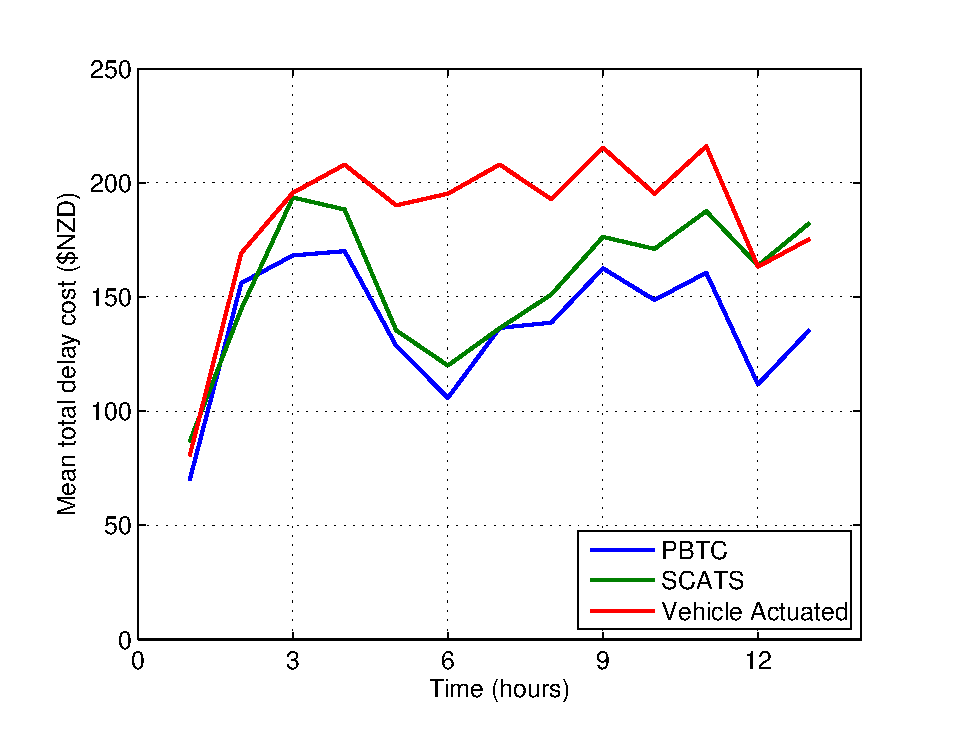
\includegraphics[scale=0.5]{vivian_victoria_delay_cost_time.eps}
  \caption{Vivian-Victoria}
  \label{delay_cost_time:sub1}
\end{subfigure}%
\begin{subfigure}{.5\textwidth}
  \centering
  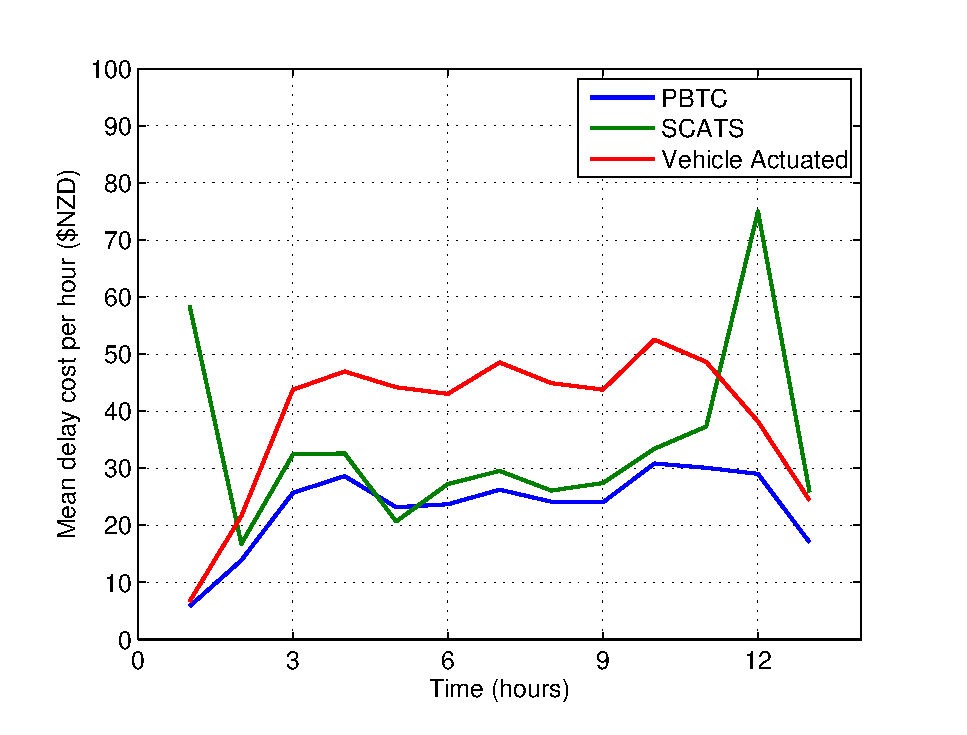
\includegraphics[scale=0.5]{courtenay_tory_delay_cost_time.eps}
  \caption{Courtenay-Tory}
  \label{delay_cost_time:sub2}
\end{subfigure}

\vspace{1cm}

\begin{subfigure}{.5\textwidth}
  \centering
  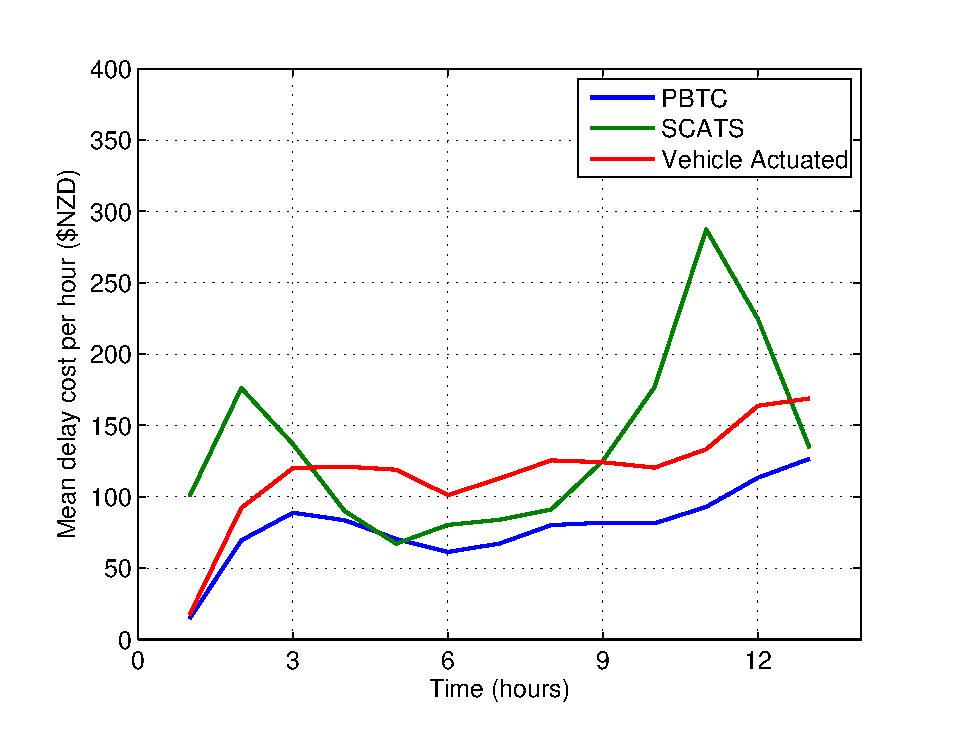
\includegraphics[scale=0.5]{karo_victoria_delay_cost_time.eps}
  \caption{Karo-Victoria}
  \label{delay_cost_time:sub3}
\end{subfigure}%
\caption[Results of measuring the mean delay cost per hour incurred for each evaluation control strategy and intersection.]{ A plot of the mean delay cost per hour for each of the PBTC, SCATS, and Vehicle Actuated control strategies as applied to each of the three evaluation intersection configurations. Each plot line displays an indication of the trend in delay cost over the period of a day. The PBTC and SCATS strategies typically achieve lower costs between 3 and 9 hours of simulation time, which is clear evidence that these control strategies can adapt to the lower traffic volumes over this time period. The Vehicle Actuated control strategy does not adapt phase times and the mean delay cost recorded per hour is significantly higher and relatively consistent; with the exception of the Karo-Victoria intersection where the Vehicle Actuated strategy performs very well suggesting that the fixed phase times of this plan were a good fit for the traffic flow at this intersection over the evaluation period. }
\label{eval:delay_cost_time}
\end{figure}

Figure \ref{eval:delay_cost_time} shows a clear illustration of the difference between the adaptive PBTC and SCATS control strategies, and the non-adaptive Vehicle Actuated strategy. The mean delay cost for both the PBTC and SCATS control strategies tends to peak both in the a.m. period between 0 and 3 hours of simulation time and the evening period beyond 9 hours of simulation time, with a period of lower mean delay cost per hour in between. The adaptive effect is most prominently displayed in Figures \ref{delay_cost_time:sub1} and \ref{delay_cost_time:sub2}, corresponding to the intersections of Victoria Street and Vivian Street and Courtenay Place and Tory Street, respectively. A greater understanding of the relationship between delay cost and traffic flow can be found by comparing these results to the trend in traffic volume over the same period, as shown in Figure \ref{eval:vehiclearrivalstime}. The observed lower volume of traffic between 3 and 9 hours of simulation time indicates lower delay costs can be achieved by the PBTC and SCATS strategies as traffic volume decreases. This is in contrast to the results of the Vehicle Actuated system, where the mean delay cost per hour is relatively consistent over the entire period of a day, evidence of the fixed, non-adaptive nature of the Vehicle Actuated strategy.

The trend in mean delay cost per hour between the PBTC and SCATS control strategies is observed to be similar over the period of evaluation at the Vivian Street and Victoria Street intersection, as shown in chart \ref{delay_cost_time:sub1} . The plot of delay cost and time for the two systems follow a similar pattern, however the PBTC system achieves consistently lower delay costs across this period. This result is evidence of the incremental adaptation algorithm used by the SCATS system to adjust phase duration. SCATS and PBTC both adjust their phase times to meet the volume of demand at an intersection, though SCATS is an incremental adjustment based on near real-time flow and the PBTC system is a direct adjustment based on vehicles present in real-time, hence adjustments made by the SCATS system affect future traffic rather than vehicles present at the time of adjustment.

In contrast, SCATS is observed to perform worse than both the PBTC and Vehicle Actuated control strategies over the peak traffic period at the intersection of Karo Drive and Victoria Street. The mean delay cost recorded by the SCATS strategy is much higher than the PBTC and Vehicle Actuated strategies between 10 and 12 hours of the evaluation period. This period is similarly explained by the incremental adaptation of the SCATS system. Traffic flow increases during this period, starting at approximately 4 p.m. (10 hours into simulation), corresponding with the sharp increase in mean total delay as the intersection becomes saturated and adaptive control is required to extend phase durations. After 11 hours of simulation time, the mean delay cost per hour recorded by the SCATS system decreases, even as the traffic flow continues to increase. This suggests that after the period of incremental adaptation, the phase times operated by SCATS eventually become more suitable for the volume of traffic recorded. 

Figure \ref{delay_cost_time:sub3} shows that the Vehicle Actuated control strategy outperforms SCATS for most of the evaluation period on the Karo Drive and Victoria Street intersection. This result supports indications that the 60 second maximum phase duration used by the Vehicle Actuated control strategy is a good fit for this intersection over the evaluation period.

\section{Incurred Stopping Cost}
\label{sec:incurred_stopping_cost}

The costs incurred by vehicles required to stop at a controlled intersection is another design metric of the PBTC system and as a result, analysis of the incurred stopping cost is included in this evaluation. Figure \ref{eval:mean_stopping_cost} shows the mean incurred stopping costs for an individual vehicle per vehicle urgency, over each of the three evaluation intersections and control strategies. 

\begin{figure}
\centering
\begin{subfigure}{.5\textwidth}
  \centering
  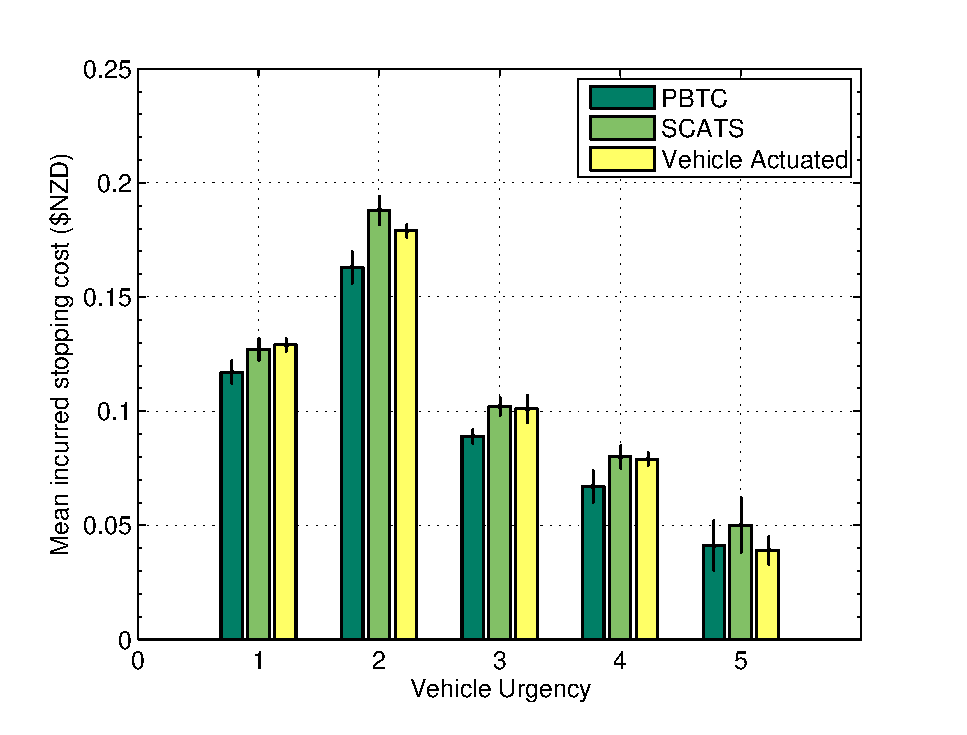
\includegraphics[scale=0.5]{vivian_victoria_approaches_stopping_cost.eps}
  \caption{Vivian-Victoria}
  \label{mean_stopping_cost:sub1}
\end{subfigure}%
\begin{subfigure}{.5\textwidth}
  \centering
  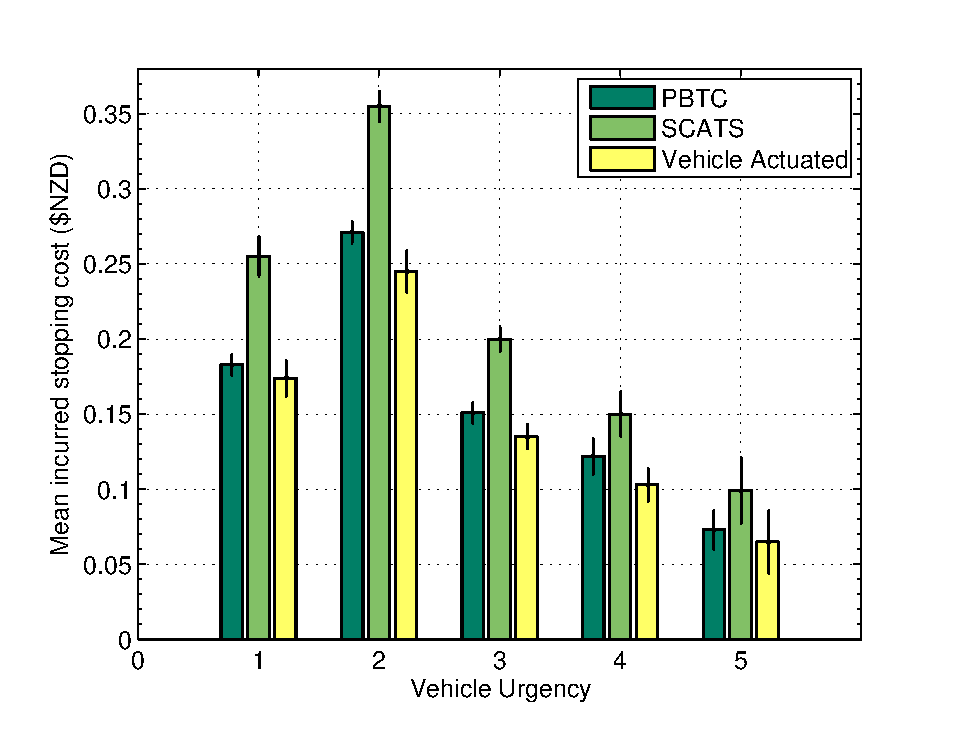
\includegraphics[scale=0.5]{courtenay_tory_approaches_stopping_cost.eps}
  \caption{Courtenay-Tory}
  \label{mean_stopping_cost:sub2}
\end{subfigure}

\vspace{1cm}

\begin{subfigure}{.5\textwidth}
  \centering
  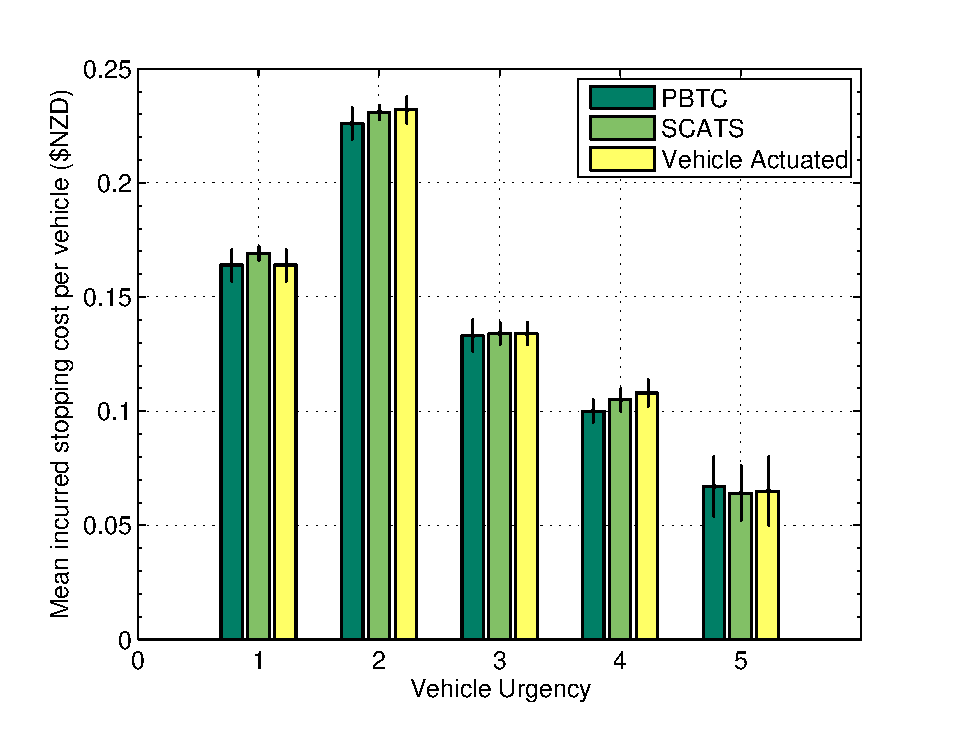
\includegraphics[scale=0.5]{karo_victoria_approaches_stopping_cost.eps}
  \caption{Karo-Victoria}
  \label{mean_stopping_cost:sub3}
\end{subfigure}%
\caption[Results of measuring the mean stopping cost incurred by individual vehicles for each evaluation control strategy and intersection.]{ A bar chart of the mean incurred stopping cost of an individual vehicle, in New Zealand Dollars, for each of the three simulated intersections. Error bars shown are representative of a single standard deviation of the mean result. The PBTC system consistently achieves lower mean stopping costs for vehicles in the simulation, although the performance of the SCATS and Vehicle Actuated systems is much more comparable than performance with respect to mean delay cost.   }
\label{eval:mean_stopping_cost}
\end{figure}

There is a consistent trend of decreasing stopping cost as urgency increases over all of the control strategies for the three evaluation intersections. This trend is accordant with the distribution of vehicle urgencies shown in Table \ref{urgencydistribution}, as the probability of an heavy vehicle with a large cost of stopping (e.g. bus or commercial truck) having a higher urgency value is comparatively low, and not possible in the case of urgency 5. The highest recorded mean stopping costs are observed for urgency 2 vehicles, which has the highest proportion of heavy vehicles. 

\begin{figure}
\centering
\begin{subfigure}{.5\textwidth}
  \centering
  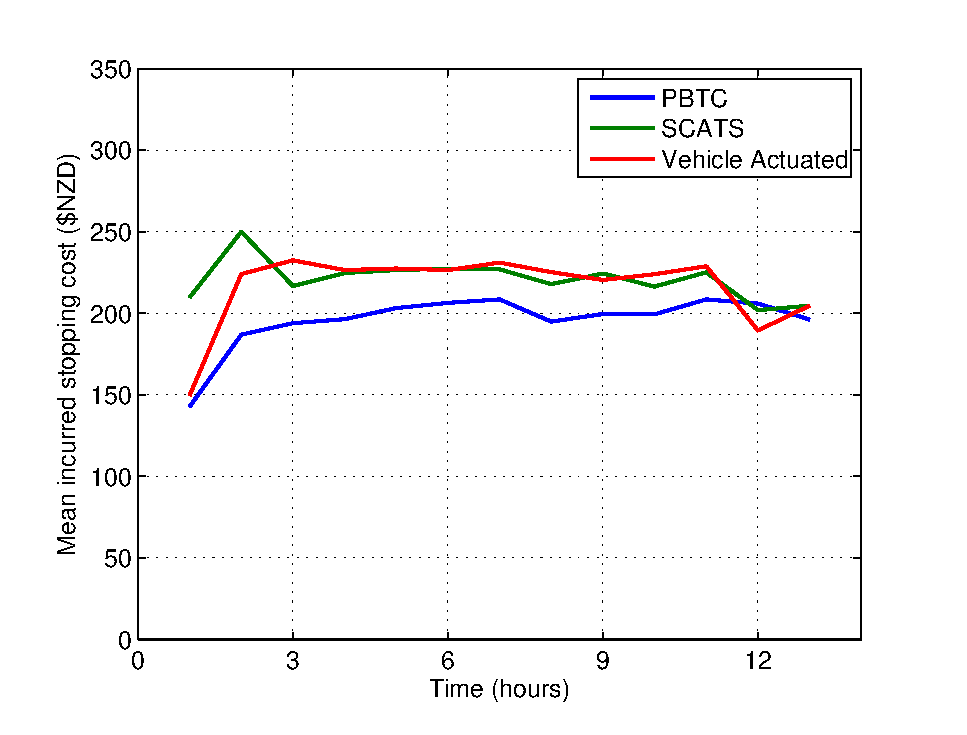
\includegraphics[scale=0.5]{vivian_victoria_stopping_cost_time.eps}
  \caption{Vivian-Victoria}
  \label{stopping_cost_time:sub1}
\end{subfigure}%
\begin{subfigure}{.5\textwidth}
  \centering
  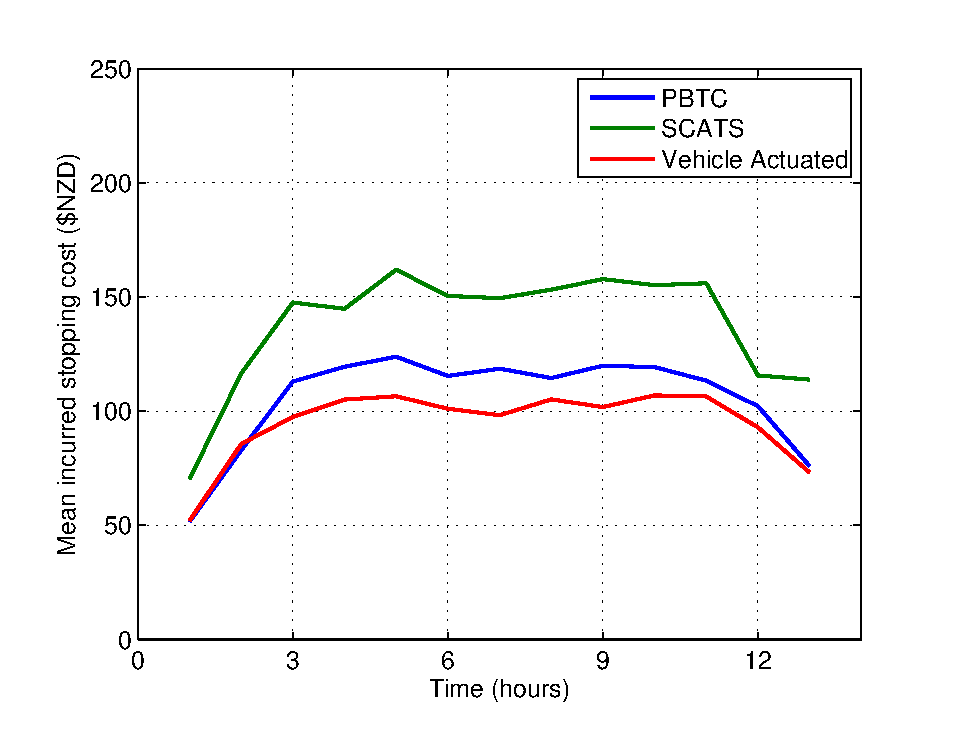
\includegraphics[scale=0.5]{courtenay_tory_stopping_cost_time.eps}
  \caption{Courtenay-Tory}
  \label{stopping_cost_time:sub2}
\end{subfigure}

\vspace{1cm}

\begin{subfigure}{.5\textwidth}
  \centering
  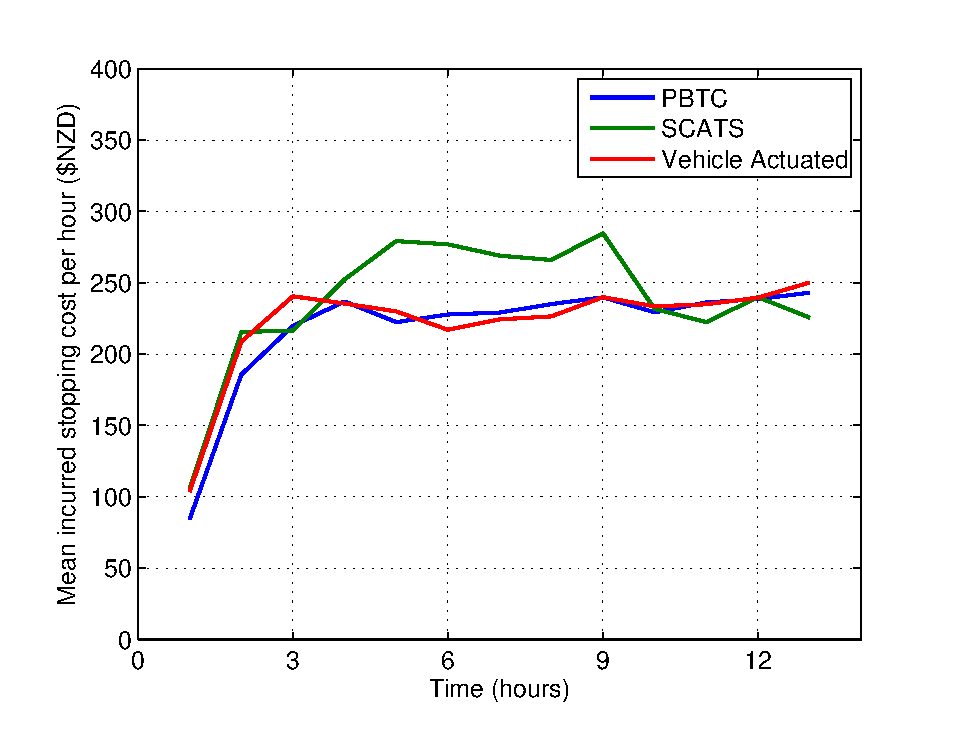
\includegraphics[scale=0.5]{karo_victoria_stopping_cost_time.eps}
  \caption{Karo-Victoria}
  \label{stopping_cost_time:sub3}
\end{subfigure}%
\caption[Results of measuring the mean stopping cost per hour incurred for each evaluation control strategy and intersection.]{ A plot of the mean incurred stopping cost per hour for each of the PBTC, SCATS, and Vehicle Actuated control strategies as applied to each of the three evaluation intersection configurations. Each plot line displays an indication of the trend in stopping cost over the period of a day.  }
\label{eval:stopping_cost_time}
\end{figure}

Figure \ref{eval:mean_stopping_cost} also shows that the PBTC control strategy performs well with regards to reducing the mean stopping cost at all three evaluation intersections, outperforming both the SCATS and Vehicle Actuated systems over a majority of the vehicle urgency values, but by only a small margin in most cases. It is important to note the cost of stopping is closely related to the speed of vehicles flowing through the system. The cost of stopping individual vehicles travelling slowly in a queue is appreciably lower than stopping freely flowing vehicles traveling at the speed limit of the area, due to the lower instantaneous velocity at the point of stopping. As a result, an inverse relationship exists between delay cost and incurred stopping cost with respect to vehicle speed. This result can be used to explain the similar performance of the SCATS and Vehicle Actuated control strategies when compared to the performance of the PBTC system. As the mean delay time per vehicle achieved by the SCATS and Vehicle Actuated strategies is greater, the length of vehicle queues is higher, resulting in relatively lower mean stopping costs.

The relationship between time of day and mean stopping cost recorded per hour is shown in Figure \ref{eval:stopping_cost_time}. The performance of the three control strategies is relatively similar over each of the three evaluation intersections, although the mean stopping cost per hour recorded by the SCATS system appears to be consistently higher over the duration of the evaluation period. The mean stopping cost per hour measured for each of the PBTC and Vehicle Actuated control strategies is similar and varies between the three evaluation intersections. Given that the mean delay time over these periods is significantly lower for the PBTC system, the lower mean stopping cost is a benefit of the strategy itself, rather than long delay/slower traffic as is the case for the SCATS and Vehicle Actuated systems.
% do we need to back this up with queue stats?

\section{Overall Incurred Costs}

The overall incurred cost of operation over the evaluation period is an important metric as the primary goal of the PBTC system is to reduce the overall operation costs by including consideration of individual vehicle costs in traffic control  decisions. Figure \ref{eval:total_cost} and Table \ref{eval:total_costs_table} show the mean and standard deviation of the total overall costs measured for 10 simulation runs on each of the simulated intersections.

The PBTC control strategy achieves the lowest mean total cost over all three simulated intersections, with between 13.7\% and 32.5\% reduction in overall costs compared to the SCATS control strategy, and 13.9\% to 19.0\% when compared to the Vehicle Actuated strategy. This result is supported by the results of the previous sections, where the PBTC control system is able to achieve the lowest mean delay times, delay costs, and incurred stopping costs for all of the simulated intersections. 

These results also show that the Vehicle Actuated control strategy outperforms SCATS with respect to the mean total cost for the evaluation period for the Courtenay-Tory and Karo-Victoria intersections. The results of Sections \ref{sec:incurred_delay_cost} and \ref{sec:incurred_stopping_cost} show that SCATS performs significantly worse than the Vehicle Actuated control strategy with respect to delay cost at the Karo-Victoria intersection and stopping cost at the Courtney-Tory intersection, respectively.

Overall delay costs for the Courtenay-Tory intersection are relatively low and as a result  the mean stopping cost per vehicle is a more significant factor that accounts for a larger proportion of the overall costs incurred during intersection operation. As previously described, the relatively poor performance of the Vehicle Actuated strategy with respect to delay time creates longer, slow-moving vehicle queues, where stopping the queue does not incur significant stopping cost for each individual vehicle and as a result the overall cost is observed to be lower than that of SCATS. Although this result appears positive for the Vehicle Actuated strategy, in practice the long delay times are undesirable and increase the potential for queues to limit the throughput of the infrastructure to the point where the network reaches a ``gridlock'' preventing queues from clearing. 

\begin{figure}
\centering
\begin{subfigure}{.5\textwidth}
  \centering
  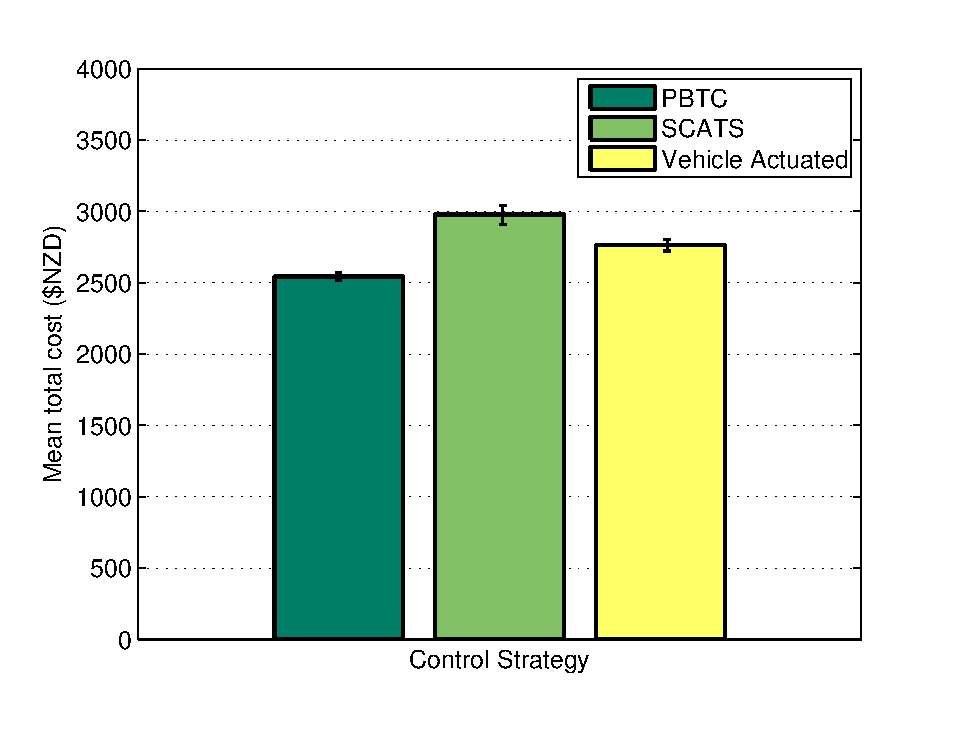
\includegraphics[scale=0.5]{vivian_victoria_approaches_total_cost.eps}
  \caption{Vivian-Victoria}
  \label{total_cost:sub1}
\end{subfigure}%
\begin{subfigure}{.5\textwidth}
  \centering
  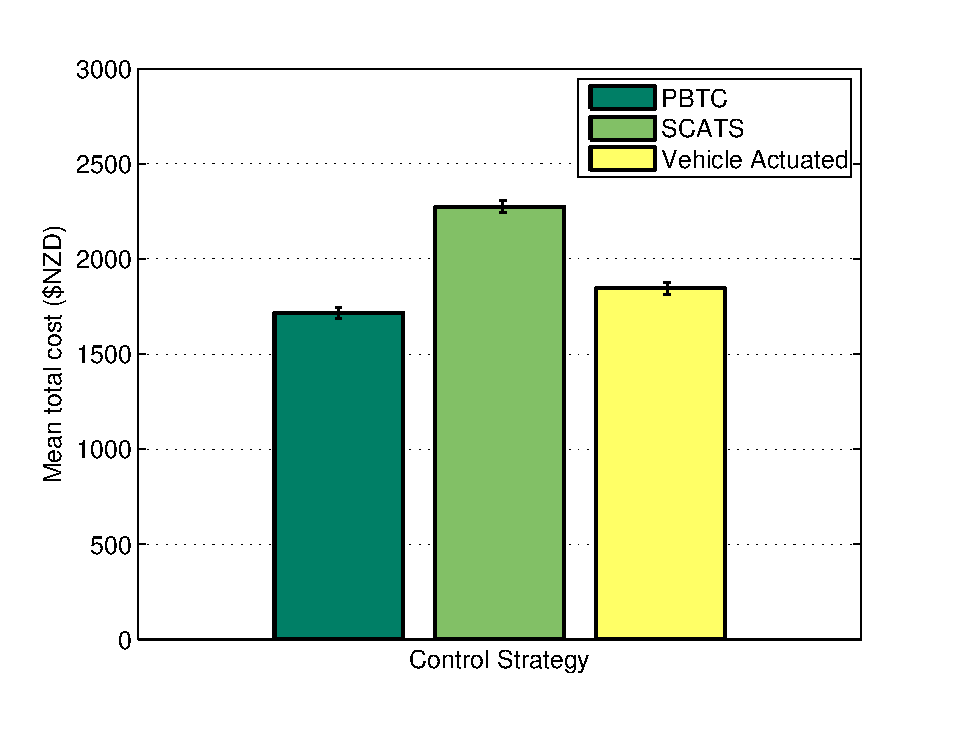
\includegraphics[scale=0.5]{courtenay_tory_approaches_total_cost.eps}
  \caption{Courtenay-Tory}
  \label{total_cost:sub2}
\end{subfigure}

\vspace{1cm}

\begin{subfigure}{.5\textwidth}
  \centering
  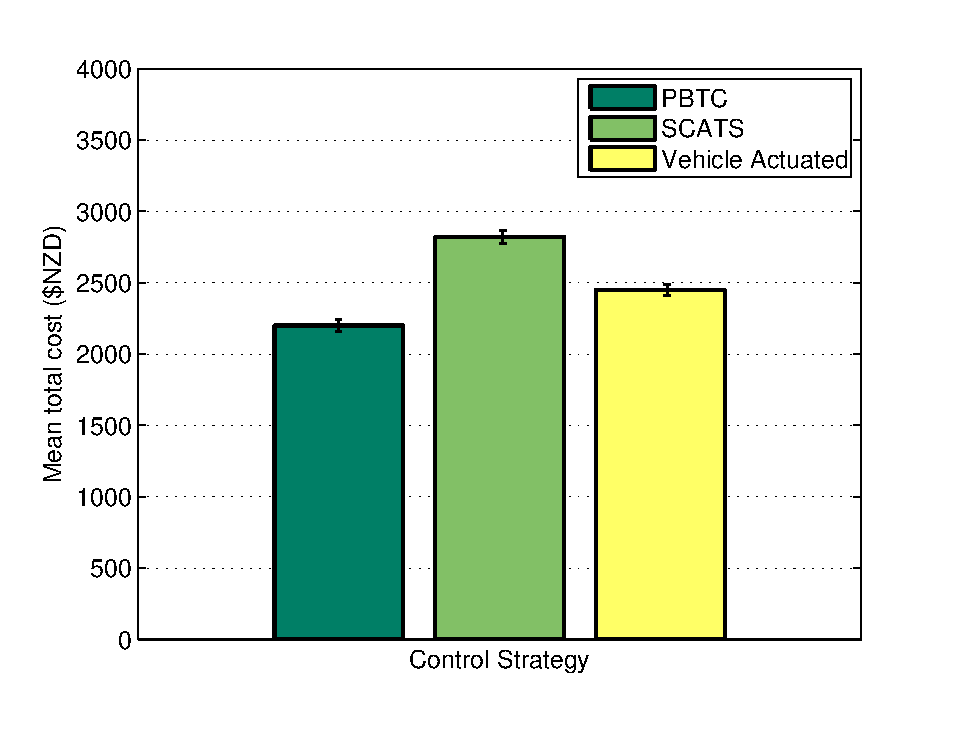
\includegraphics[scale=0.5]{karo_victoria_approaches_total_cost.eps}
  \caption{Karo-Victoria}
  \label{total_cost:sub3}
\end{subfigure}%
\caption[Results of measuring the overall costs incurred each evaluation control strategy and intersection.]{A bar chart of the mean total cost (NZD) of ten simulation runs, and percentage difference relative to the performance of the PBTC system for each of the three control strategies and intersection examples used for evaluation. Error bars shown are representative of a single standard deviation of the mean result. The PBTC control system consistently achieves a lower mean total cost compered to the SCATS and Vehicle Actuated control strategies for each of the intersections evaluated. }
\label{eval:total_cost}
\end{figure}

The results presented in this experimental evaluation support the notion of a cost tradeoff between stopping a currently flowing traffic approach and delaying all other competing approaches, the design basis of the PBTC system. To analyse how each of the strategies evaluated balances these cost values, Figure \ref{eval:cycle_durations} shows a plot of the mean cycle duration for each of the three control strategies over the period of each simulation. It is expected that during periods of high demand, longer cycle lengths are desirable to clear queues and reduce overall delay. Of each of the three systems, the PBTC control strategy typically operates the longest cycle durations.

Figure \ref{cycle_durations:sub1} shows an example of the different phase duration strategies operated by each of the control strategies. Between 8 and 12 hours, the PBTC control strategy fluctuates sharply between 130 and 160 seconds. As the PBTC control algorithm adapts to real-time traffic demand based on vehicles present and within range, more pronounced peaks of extended duration are expected. In contrast, the Vehicle Actuated control strategy has very little cycle duration variance and the recorded cycle duration does not exceed 110 seconds for the same period, due to the fixed phase durations operated by this strategy. The same period also shows evidence of incremental adaptation of the SCATS control algorithm, as the mean cycle duration increases by 40 seconds over a 2 hour period. 

Small periods of long cycle durations for each of the systems are observed during times of low traffic demand, where a phase is extended beyond its typical duration because no competing phases are demanded. This is most obvious on the Courtney-Tory and Karo-Victoria intersections, where the trend of mean cycle duration for SCATS fluctuates over the middle of the day. Referring to the trend in vehicle arrivals displayed in Figure \ref{eval:vehiclearrivalstime} it is shown that at least one of the approaches to each intersection recorded relatively low traffic volumes at this time, explaining the lack of competing demand and extended phase durations.

The mean cycle durations operated by SCATS for the Courtenay-Tory intersection explains the observed period of significantly high mean delay costs for individual vehicles shown in \ref{delay_cost_time:sub2}. Figure \ref{cycle_durations:sub2} shows that over this period the mean cycle durations operated by SCATS were very low when compared to the PBTC and Vehicle Actuated strategies. The lower cycle duration over this period results in a larger number of phase changes and greater proportion of lost effective green time on both approaches, leading to longer queues and the observed jump in mean delay cost incurred. 

\begin{table}[]
\begin{center}
\begin{tabular}{llrlrlr}
\toprule
 & \multicolumn{2}{c}{Vivian-Victoria} & \multicolumn{2}{c}{Courtenay-Tory} & \multicolumn{2}{c}{Karo-Victoria} \\
 \cmidrule(lr){2-3}
 \cmidrule(lr){4-5}
  \cmidrule(lr){6-7}
Strategy &  Total Cost & \Delta\% & Total Cost & \Delta\% & Total Cost & \Delta\% \\
\midrule
PBTC & 4336.15 (\pm 34.8) &  & 1696.96 (\pm 31.2) & & 4051.84 (\pm 50.9) & \\
SCATS & 4928.21 (\pm 38.9) & +13.7\% & 2294.13 (\pm 31.1) & +35.2\%  & 4859.15 (\pm 48.0) & +19.9\% \\ 
VA & 5161.13 (\pm 27.5) & +19.0\% & 1969.76 (\pm 18.1) & +16.1\% & 4615.98 (\pm 45.3) & +13.9\% \\
\bottomrule
\end{tabular}
\end{center}
\caption{ Mean total cost (NZD) of ten simulation runs, and percentage difference relative to the performance of the PBTC system for each of the three control strategies and intersection examples used for evaluation. Mean total cost error is a single standard deviation of the mean total cost for ten simulation runs. The PBTC control system achieves between 13.7\% and 35.2\% reduction of the total costs of operation over the 13-hour evaluation period. }
	\label{eval:total_costs_table}
\end{table}

\begin{figure}
\centering
\begin{subfigure}{.5\textwidth}	
  \centering
  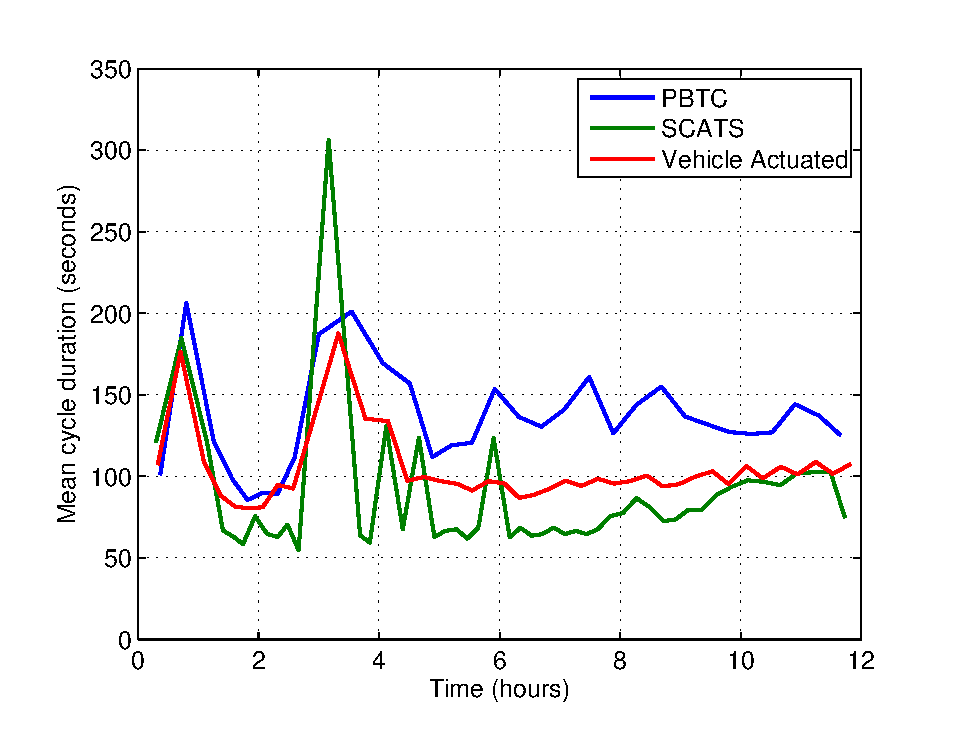
\includegraphics[scale=0.5]{vivian_victoria_cycle_durations.eps}
  \caption{Vivian-Victoria}
  \label{cycle_durations:sub1}
\end{subfigure}%
\begin{subfigure}{.5\textwidth}
  \centering
  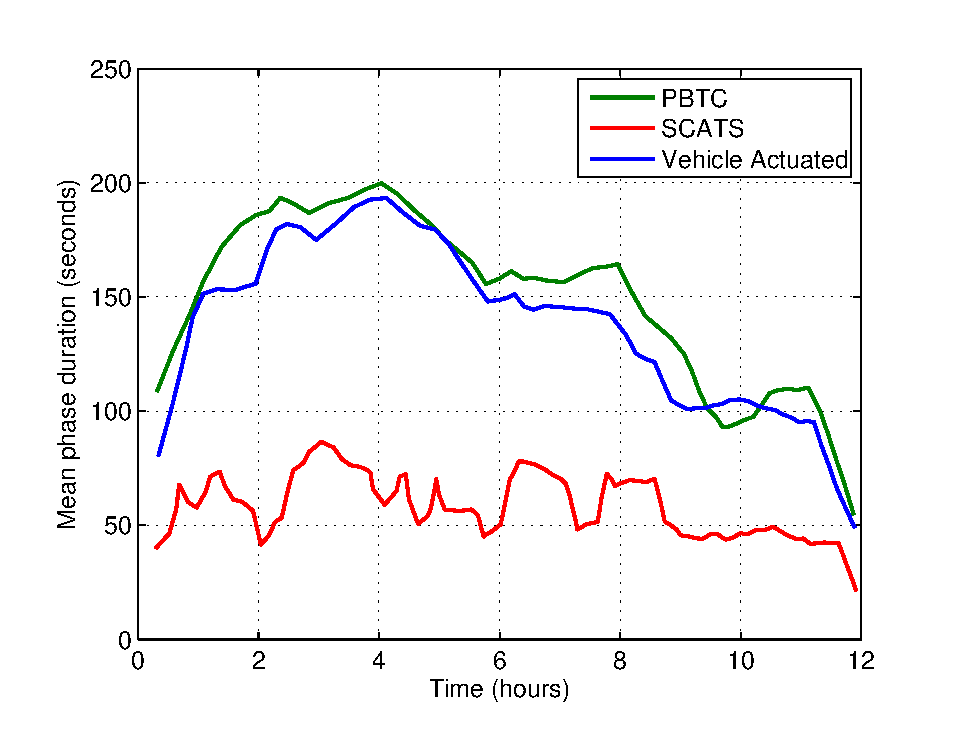
\includegraphics[scale=0.5]{courtenay_tory_cycle_durations.eps}
  \caption{Courtenay-Tory}
  \label{cycle_durations:sub2}
\end{subfigure}

\vspace{1cm}

\begin{subfigure}{.5\textwidth}
  \centering
  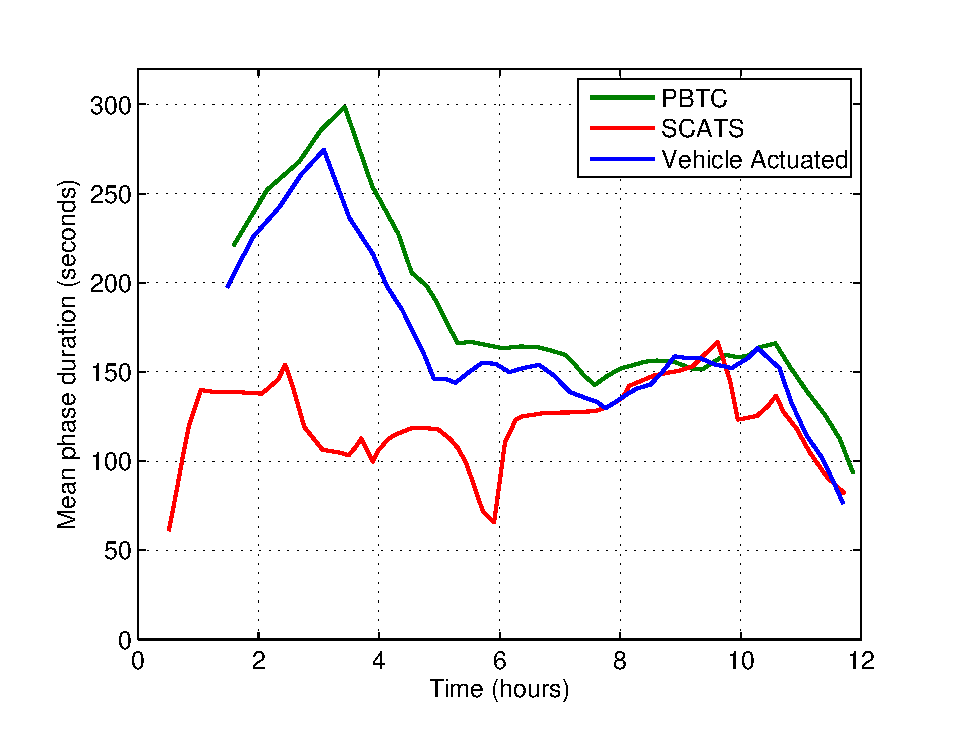
\includegraphics[scale=0.5]{karo_victoria_cycle_durations.eps}
  \caption{Karo-Victoria}
  \label{cycle_durations:sub3}
\end{subfigure}%
\caption[Results of measuring the mean cycle duration per hour for each control strategy and intersection.]{ A plot of the mean cycle duration per hour, measured in seconds for each of the PBTC, SCATS, and Vehicle Actuated control strategies over each of the simulated intersections. The cycle duration is calculated by adding the durations of each pair of phases in the system. The PBTC and Vehicle Actuated strategies are closely related as they both operate on the basis of real-time vehicle detections/communication broadcasts. Large peaks are observed whenever periods of low traffic volume cause a phase to be extended due to no competing demand.  }
\label{eval:cycle_durations}
\end{figure}

\section{Discussion}

The results presented in this chapter show the design of the PBTC control algorithm successfully reduces time spent delayed, costs incurred by delay, and costs incurred by stopping compared to the SCATS and Vehicle Actuated control strategies for all of the simulated intersections used for evaluation. In addition, the PBTC control system is able to prioritise vehicles based on their urgency, decreasing the delay time for vehicles with a higher relative urgency of travel.

\subsection{Validity}

A considerable effort has been made to ensure the validity and applicability of the results generated by this project. Design decisions related to the traffic priority model used to estimate journey costs; software design of PBTSim for simulation; and design and implementation of the PBTC control strategy, Vehicle Actuated control strategy, and SCATS representation; have been carefully considered to model realistic traffic scenarios. Threats to validity are based upon the assumptions made when designing estimate models, and representation of the traffic composition and SCATS behaviour during experimental evaluation.

\subsubsection{Priority Modeling for Cost Estimation}

The priority model designed during this project was required for the design and development of the PBTC system, and evaluation of the performance of the three control strategies tested during experimental evaluation. Cost of delay and cost of stopping are the primary components of this model. These costs are quantifiable and based on existing implicit costs incurred by motorists on real-world road networks. 

To calculate the cost of delay, a model has been designed based on the New Zealand Transport Agency recommended figure of \$26.20 New Zealand Dollars per vehicle hour, as opposed to an arbitrarily designed numerical value with no research as the basis of quantification. For the purposes of this project, this value is assumed to be correct for all vehicles on New Zealand roads. 

To calculate the cost of stopping a vehicle, a physics based fuel consumption model has been designed based on the kinetic energy required to accelerate a vehicle to a given speed, and the amount of speed effectively ``lost'' when a vehicle is forced to stop their journey at a controlled intersection. This model is limited by lack of consideration of different engine efficiencies, power to consumption ratios of different vehicle gears, and driver behaviours; all of which can improve or deteriorate the costs of fuel consumption involved in a forced stop. The separation of simulation vehicles into fixed, light or heavy classes is a significant simplification which doesn't accurately model realistic traffic composition on New Zealand roads. It is expected that more sophisticated modeling may influence the cost values produced by experimentation, but consistently, so the relative performance of each of the control strategies will not be significantly affected.

\subsubsection{SCATS Log Data}

 This project relies on the data contained in log files produced by the SCATS system operating in Wellington City and provided by the Wellington City Council for simulation of traffic volume and experimental evaluation of the performance of the SCATS control strategy with regards to delay and stopping cost incurred with prioritised traffic.
 
The use of logged SCATS data introduces threats to the validity of experimental results. The SCATS log files are poorly labeled and can contain up to four detectors per approach. It is often unclear exactly which detectors are recording logged data without specific knowledge of the configuration on a per intersection basis. The software package designed to parse SCATS logs within PBTSim assumed that all approach data for each labelled approach identified of interest was relevant, with the exception of the Courtenay-Tory intersection where this behaviour was overridden to exclude data that was known to relate to the omitted turning lanes of both streets. The accuracy of detector data in the SCATS log file for the Karo-Victoria intersection should be doubted, as the SCATS representation consistently performed worse on this intersection compared to Vivian-Victoria and Courtenay-Tory across all evaluation metrics, and the measured flow rate at Victoria Street was significantly less than expected.

The SCATS log data is also used to set the phase times for the SCATS system during simulation. While these phase durations can be expected to be correct, because vehicle arrivals are simulated using the Poisson process there is no certainty that the vehicles present at any instantaneous moment of simulation are reliably reflective of the real-world demand. More robust evaluation is suggested as an area of future work for this project.


